\documentclass[a0paper,25pt]{tikzposter} %Options for format can be included here
\usepackage{pgfplots}
\usepackage{amsmath}
\usepackage{amsfonts}
\usepackage{amssymb}
\usepackage{amsthm}

\newtheorem*{mydef}{Definition}
\newtheorem{theorem}{Theorem}

\renewcommand\Re{\mathop{\rm Re}\nolimits}
\renewcommand\Im{\mathop{\rm Im}\nolimits}



 % Title, Author, Institute
\title{
\vbox{
Inverse problems for Sturm-Liouville operators  
with Bessel-type singularity inside an interval
}
}
\author{Alexey Fedoseev}
\institute{Saratov State University, Russia}
%\titlegraphic{LogoGraphic Inserted Here}

 %Choose Layout
%\usetheme{Default}

%\usetheme{Board}
%\usecolorstyle{Russia}
\tikzposterlatexaffectionproofoff

\begin{document}

 % Title block with title, author, logo, etc.
\maketitle

\begin{columns}

\column{0.5}


\block{}{
The inverse spectral problems theory was discovered and introduced by Soviet-Armenian astrophysicist Victor Ambartsumian.

Just after his graduation from the University of Leningrad he was interested in what degree do the eigenvalues of an ordinary differential operator determine the functions and parameters entering into that operator? Ambartsumian published in 1929 in Zeitschrift f\"ur Physik a paper which contained the statement of the general problem and the proof of the theorem that among all strings the homogeneous string is uniquely defined by the set of its oscillation-frequencies.
%does the empirical data of atomic physics (the frequencies of spectral lines, the transition probabilities, etc.) define the system of laws and rules of quantum mechanics or more specifically the form of the Schr\"odinger equation?
Consider the boundary value problem
\begin{equation}
-y''+q(x)y=\lambda y, \quad y'(0)=y'(\pi)=0.
\label{Ambartsumian}
\end{equation}
Clearly, if $q(x)=0$ a.e. on $(0,\pi),$ then the eigenvalues
of \eqref{Ambartsumian} have the form $\lambda_n=n^2$,$n\ge 0$.
Ambartsumian proved the inverse assertion:

\innerblock[titleleft]{Theorem}
{If the eigenvalues of \eqref{Ambartsumian} are
$\lambda_n=n^2,\;n \ge 0,$ then $q(x)=0$ a.e. on $(0,\pi)$.}

During the fifteen years nobody has taken notice of that paper. However in 1944 that work was found by Swedish mathematicians who have obtained many interesting results related to the ''inverse Sturm-Liouville problem`` and thus that paper became the foundation of an entire discipline.
%(Ambartsumian said ``when an \textit{astronomer} is publishing a \textit{mathematical} paper in a \textit{physical} journal, he cannon expect to attract too many readers'')
}

\block{What is Inverse Problems?}{
\innerblock{What is Inverse Problems?}{Solution of an inverse problem entails determining unknown causes, based on observation of their effects.}
Solution of an inverse problem entails determining unknown causes, based on observation of their effects.

Inverse problem: causes -> consequences (observations, effects, results)

Direct problem: consequences -> causes

\begin{tikzfigure}[A figure can be made withoes not work]

\includegraphics[scale=1]{Neptune.pdf}
\end{tikzfigure}

}



\column{0.5}

\block{First Result in Spectral Inverse Problems Theory}{

TAKE FROM document.pdf Part 2 Inverse problems!!!!!!!!!!!!!!!!11
!!!!!!!!!!!!!!!!!!!!!!!1

\


%The first result in the inverse problem theory is due to Ambartsumian (Ambartsumian V., \"Uber eine Frage der Eigenwerttheorie., Zeit. f\"ur Phys., 53 (1929), pp. 690--695).
%Consider the boundary value problem $L(q(x),0,0),$ i.e.
%\begin{equation}
%-y''+q(x)y=\lambda y, \quad y'(0)=y'(\pi)=0.
%\label{Ambartsumian}
%\end{equation}
%Clearly, if $q(x)=0$ a.e. on $(0,\pi),$ then the eigenvalues
%of \eqref{Ambartsumian} have the form $\lambda_n=n^2$,$n\ge 0$.
%Ambartsumian proved the inverse assertion:
%
%\innerblock[titleleft]{Theorem}
%{If the eigenvalues of \eqref{Ambartsumian} are
%$\lambda_n=n^2,\;n \ge 0,$ then $q(x)=0$ a.e. on $(0,\pi)$.}





%Первый результат в теории обратных спектральных задач принадлежит советскому ученому, основателю теоретической астрофизики В.А. Амбарцумяну \cite{Ambarzumian1929}. Интересен вопрос о том, как он пришел к обратной задачи. В 1926 году Э. Шредингер опубликовал работы \cite{Schroedinger1926part1,Schroedinger1926part2,Schroedinger1926part3,Schroedinger1926part4,Schroedinger1926Heisenberg} по волновой механике. Он показал, что вопрос исследования энергетических уровней системы приводит к решению задач нахождения собственных значений некоторых дифференциальных уравнений.
%% , то есть спектр энергетических уровней может быть получен с помощью вычисления спектра собственных значений этих уравнений.
%% В.А. Амбарцумяна интересовало объяснение происхождения спектров атомов.
%В астрофизике спектральный анализ атомов является одним из основных методов исследования небесных объектов. В.А. Амбарцумян хотел выяснить можно ли по наблюдаемым спектрам атомов однозначно узнать о строении и состоянии атома, что и является ``обратной'' задачей. Оказалось, что решение этой нелинейной задачи в общем случае весьма трудно.
%% Тогда Амбарцумян упростил задачу: как частоты колебаний струны зависят от ее диаметра и других ее параметров? Но данная задача так же оказалась очень трудной.
%Тогда он рассмотрел частный случай: можно ли утверждать, что система собственных частот, характерная для однородной струны, свойственна только ей и однозначно определяет ее среди всех струн? Ему удалось разрешить эту проблему и сформулировать следующий результат\cite{Ambarzumian1929} для уравнения Штурма-Лиувилля
%\begin{equation}
%-y''+q(x)y=\lambda y.
%\label{intro:SLeq}
%\end{equation}
%Здесь $\lambda$ - спектральный параметр, $q(x)$, $x\in(0,\pi)$ - вещественная интегрируемая функция.
%%, $q(x)\in L_2(0,\pi)$.
%В.А. Амбарцумян показал, что если краевая задача для уравнения \eqref{intro:SLeq} с граничными условиями $y'(0)=y'(\pi)=0$ имеет собственные значения $\lambda_n=n^2$, $n\geq 0$, то $q(x)=0$. Однако этот результат является исключительным - в общем случае задания одного спектра недостаточно для восстановления потенциала $q(x)$.

=================================================

The field of inverse problems was first discovered and introduced by Soviet-Armenian physicist, Viktor Ambartsumian.

While still a student, Ambartsumian thoroughly studied the theory of atomic structure, the formation of energy levels, and the Schr\"odinger equation and its properties, and when he mastered the theory of eigenvalues of differential equations, he pointed out the apparent analogy between discrete energy levels and the eigenvalues of differential equations. He then asked: given a family of eigenvalues, is it possible to find the form of the equations whose eigenvalues they are? Essentially Ambartsumian was examining the inverse Sturm-Liouville problem, which dealt with determining the equations of a vibrating string. This paper was published in 1929 in the German physics journal Zeitschrift f\"ur Physik and remained in obscurity for a rather long time (Ambartsumian V., {\it\"Uber eine Frage der Eigenwerttheorie.}, Zeit. f\"ur Phys., 53 (1929), pp. 690--695). Describing this situation after many decades, Ambartsumian said, "If an astronomer publishes an article with a mathematical content in a physics journal, then the most likely thing that will happen to it is oblivion."

Nonetheless, toward the end of the Second World War, this article, written by the 20-year-old Ambartsumian, was found by Swedish mathematicians and formed the starting point for a whole area of research on inverse problems, becoming the foundation of an entire discipline.
}

%\block{}{
%\begin{tikzfigure}[A figure can be made withoes not work]
%
\includegraphics[scale=1]{Neptune.pdf}
%\end{tikzfigure}
%}

\end{columns}



 \begin{columns}

 % FIRST column
\column{0.5}% Width set relative to text width


\block{jkhkjh}{
Let the function $\Phi(x,\lambda)$ be a solution of \eqref{initeq} under conditions
\[
\Phi(0,\lambda)=1, \quad\Phi(x,\lambda)=O(e^{i\rho x}),\quad x\to\infty. %\quad \rho\in\Omega.
\]
where $\Im\rho\geq0$, $\rho\neq0$.

WHAT IS ${\cal L}$??????
%$\Phi(0,\lambda)=1$, $\Phi(x,\lambda)=O(\exp(i\rho x))$, $x\to\infty$, $\rho\in\Omega$. 
\innerblock{}{
Function $\Phi(x,\lambda)$ is called the \textit{Weyl solution} for ${\cal L}$.
}
\innerblock{}{
The function $M(\lambda):=\Phi'(0,\lambda)$ is called the {\it Weyl function} for ${\cal L}$.
}


\innerblock[titleleft]{Inverse Problem}{
Recover $q(x)$ by the given Weyl function $M(\lambda)$.
}
}


 




%\block{hghgjhg}{
%\begin{tikzfigure}[A figure can be made withoes not work]
%
\includegraphics[scale=1]{Neptune.pdf}
%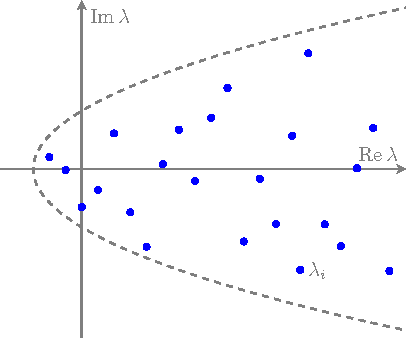
\includegraphics[scale=1]{spectra.pdf}
%\begin{tikzpicture}[scale=1]
%\draw [->, color=gray,thick] (0,0) node[below] {$0$}-- (5,0) node[below] {$x$};
%\node[shape=circle,fill=red,scale=0.3] at (2,0) {};
%\node[below,color=gray] at (2,-0.1) {$a$};
%\end{tikzpicture}
%\end{tikzfigure}
%}

\block{hgjhgjhgjhg}{
An interesting kind of generalization of Bessel equation is ...
It can be easily obtained by taking a substitution...
}
\block{Object}{
Consider the differential equation
\begin{equation}
\ell y = -y''+\Big(\frac{\nu_0}{(x-a)^2}+q(x)\Big)y=\lambda y,\quad x>0,
\label{initeq}
\end{equation}
on the half-line with a Bessel-type singularity at an interior point $a>0$. 
\begin{tikzfigure}[Some caption]
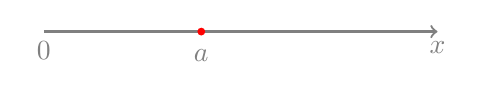
\begin{tikzpicture}[scale=1]
\draw [->, color=gray,thick] (0,0) node[below] {$0$}-- (5,0) node[below] {$x$};
\node[shape=circle,fill=red,scale=0.3] at (2,0) {};
\node[below,color=gray] at (2,-0.1) {$a$};
\end{tikzpicture}
\end{tikzfigure}
Here $q(x)$ is a complex-valued function and $\nu_0$ is a complex number. Let $\nu_0=\nu^2-1/4$ and to be definite, we assume that  $Re\,\nu>0,$ $\nu\neq 1,2,\ldots$ (the other cases require minor modifications). We also assume that $q(x)|x-~a|^{\min(0,1-2Re\,\nu)} \in L(0,T)$ for some $T>a$ and $q(x)\in L(T,\infty)$. We denote the class of such functions $q(x)$ by $W$.

CHANGE THIS!!!!!!!!!!

The paper deals with the boundary value problem  ${\cal L=L}(q)$ for differential equation \eqref{initeq} with the Dirichlet boundary condition $y(0)=0$ and an additional \textit{matching conditions} near the singular point $x=a$. We consider in some sense arbitrary matching conditions with a transition matrix $A=[a_{jk}]_{j,k=1,2},$ that connects solutions of \eqref{initeq} in a neighbourhood of the singular point (for details, see Section 2). 

CHANGE THIS!!!!!!!!!!

WHAT IS matching conditions!

WHAT IS WEYL FUNCTION!
}

\column{0.5}
 %Second column with first block's top edge aligned with with previous column's top.
\block{What is Matching Conditions?}{Let $\lambda=\rho^2$ and $\mathrm{Im}\,\rho\geq0$. Consider the functions
\[
C_j(x,\lambda)=(x-a)^{\mu_j} \sum^\infty_{k=0} c_{jk}(\rho (x-a))^{2k} ,\; j=1,2,
\]
where $c_{10}c_{20}=(2\nu)^{-1}$,
\[
\mu_j=(-1)^j\nu+1/2,\, c_{jk}=(-1)^k c_{j0}
\,\Big( \prod^k_{s=1} ((2s+\mu_j)(2s+\mu_j-1)-\nu_0)\Big)^{-1}.
\]
Here and below $z^{\mu}=\exp(\mu(\mbox{ln}|z|+i\arg z))$, $\arg z \in (-\pi, \pi]$. If $x>a$ or $x<a$ then the functions
 $C_j(x,\lambda)$ are solutions of \eqref{initeq} with $q(x)\equiv 0$. Let the functions $s_j(x,\lambda)$, $j=1,2$ be solutions of the following integral equations for $x>a$ and $x<a$: 
\[
s_j(x,\lambda)=C_j(x,\lambda)+\int^x_{a} g(x,t,\lambda)q(t)s_j(t,\lambda)\,dt,
\]
where $g(x,t,\lambda)=C_1(t,\lambda)C_2(x,\lambda)-C_1(x,\lambda)C_2(t,\lambda)$. For each fixed $x$ the functions $s_j(x,\lambda)$ are entire in $\lambda$ of order 1/2 and form a fundamental system of solutions of \eqref{initeq}. Moreover 
\begin{equation}
\det[s_j^{(m-1)}(x,\lambda)]_{j,m=\overline{1,2}}\equiv 1. 
\label{detsj}        
\end{equation} 

Let $A=[a_{jk}]_{j,k=1,2}$, $\det A\ne 0$ be a given matrix with complex numbers $a_{jk}$. We introduce the functions  $\{\sigma_j(x,\lambda)\}_{j=1,2}$, $x\in J_{-}\cup J_{+}$, $J_{\pm}=\{\pm (x-a)>0\}$ by the formula
\begin{equation*}
\sigma_j(x,\lambda)=\left\{
\begin{array}{ll}
s_j(x,\lambda), & x\in J_{-},\\
\sum\limits_{k=1}^{2}a_{kj}s_k(x,\lambda),&  x\in J_{+}.
\end{array}\right.
\label{sigmajinsk}
\end{equation*}
The fundamental system of solutions $\{\sigma_j(x,\lambda)\}$ is used to match solutions in a neighborhood of the singular point  $x=a$. It follows from \eqref{detsj} that
\begin{equation}
\det[\sigma_j^{(m-1)}(x,\lambda)]_{j,m=1,2}\equiv
\left\{ \begin{array}{ll}
1,\quad & x\in J_{-}, \\ \det A,\quad & x\in J_{+}.
\end{array}\right. 
\label{detsigmaj}                
\end{equation}

We introduce numbers $\xi_{jk}$, $j,k=1,2$ by
\begin{equation}
\left[ \begin{array}{ll}
\xi_{11} & \xi_{12} \\ \xi_{21} & \xi_{22}
\end{array}\right]= \frac{1}{2\sin\pi\nu}
\left[ \begin{array}{ll}
-a_{11}e^{2\pi i\nu}+a_{22}e^{-2\pi i\nu} & -i(a_{11}e^{\pi i\nu}-a_{22}e^{-\pi i\nu}) \\
-i(a_{11}e^{\pi i\nu}-a_{22}e^{-\pi i\nu}) & a_{11}-a_{22} 
\end{array}\right] .    
\label{ksimatrix}
\end{equation}       
The behaviour of the spectrum of the boundary value problem ${\cal L}$ depends on the numbers $\xi_{jk}$. We consider the most difficult special case in which $|\xi_{jj}|>|\xi_{12}|>0$, since in this case the discrete spectrum is unbounded and essential qualitative modifications in the investigation of the direct and inverse problems are arised. 
To be definite we set $a_{12}=0$ (the other case requires minor modifications).
\begin{tikzfigure}[A figure can be made withoes not work]
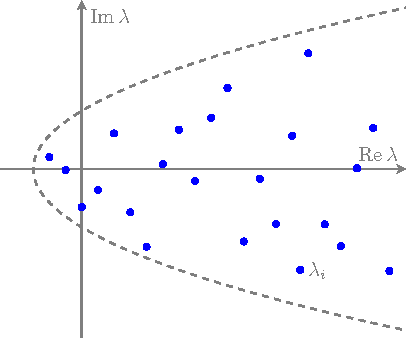
\includegraphics[scale=1]{spectra.pdf}
\end{tikzfigure}
}

\block{Using Method of Spectral Mappings}{
\innerblock[titleleft]{Uniqueness Theorem}{
%If $M(\lambda)=\widetilde M(\lambda)$, then $q(x)=\tilde q(x)$ almost everywhere for $x>0$. Thus, the Weyl function uniquely determines the boundary value problem $\cal L$.
The Weyl function uniquely determines the boundary value problem $\cal L$.
}
}



 \end{columns}

\end{document}

 \begin{columns}

 % FIRST column
\column{0.6}% Width set relative to text width

\block{Large Column}{Text\\Text\\Text Text Text}
\note{Note with default behavior}
\note[targetoffsetx=12cm, targetoffsety=-1cm, angle=20, rotate=25]
{Note \\ offset and rotated}

 % First column - second block
\block{Block titles with enough text will automatically obey spacing requirements }
{Text\\Text}

 % First column - third block
\block{Sample Block 4}{T\\E\\S\\T}

 % SECOND column
\column{0.4}
 %Second column with first block's top edge aligned with with previous column's top.

 % Second column - first block
\block[titleleft]{Smaller Column}{Test}

 % Second column - second block
\block[titlewidthscale=0.6, bodywidthscale=0.8]
{Variable width title}{Block with smaller width.}

 % Second column - third block
\block{}{Block with no title}

 % Second column - A collection of blocks in subcolumn environment.
\begin{subcolumns}
    \subcolumn{0.27} \block{1}{First block.} \block{2}{Second block}
    \subcolumn{0.4} \block{Sub-columns}{Sample subblocks\\Second subcolumn}
    \subcolumn{0.33} \block{4}{Fourth} \block{}{Final Subcolumn block}
\end{subcolumns}

 % Bottomblock
\block{Final Block in column}{
    Sample block.
}
\end{columns}




%\block[titleleft, titleoffsetx=2em, titleoffsety=1em, bodyoffsetx=2em,%
% bodyoffsety=-2cm, roundedcorners=10, linewidth=0mm, titlewidthscale=0.7,%
% bodywidthscale=0.9, bodyverticalshift=2cm, titleright]
%{Block outside of Columns}{Along with several options enabled}

\end{document}



\endinput
%%
%% End of file `tikzposter-template.tex'.
